% Each clue is marked [write] or [say]: whether players must write their
% response before ringing in, or can just say it. The game board shows
% this on the clue screen; the PDF shows it only with the writesay option.
\documentclass{article}
% Which PDF to make (the web game ignores this):
%   questions  clues only, e.g. a study sheet for students
%   answers    clues and responses
%   solutions  clues, responses, and worked solutions
% Add any of these, separated by commas, e.g. [solutions, writesay]:
%   writesay   show each clue's [write]/[say] mark (for you, not students)
%   board      always show the board overview (even with questions)
%   noboard    never show the board overview
\usepackage[solutions,writesay]{../jeopardy}

\gametitle{Multivariable Calculus}

% Notation used in the course notes
\newcommand{\bvec}[1]{\vec{\mathbf{#1}}}
\newcommand{\uveci}{\boldsymbol{\hat{\imath}}}
\newcommand{\uvecj}{\boldsymbol{\hat{\jmath}}}
\newcommand{\uveck}{\boldsymbol{\hat{k}}}
\newcommand{\dotprod}{\cdot}

\begin{document}

%======================================================================
\begin{category}{Vectors and Surfaces}

  \begin{clue}[say]
    It is the length of the vector $\bvec{a}-\bvec{b},$ where $\bvec{a} = \langle1,3\rangle$ and $\bvec{b} = \langle5,2\rangle.$
  \response
    What is $\sqrt{17}$?
  \solution
    We compute
    \[
    \bvec{a}-\bvec{b}=\langle 4,\,-1\rangle.
    \]
    So,
    \[
    \left|\bvec{a}-\bvec{b}\right|=\sqrt{4^2+(-1)^2}=\sqrt{17}.
    \]
  \end{clue}

  \begin{clue}[say]
    It is the value of $a$ that makes the vectors $\langle a,3\rangle$ and $\langle4,5\rangle$ orthogonal.
  \response
    What is $-\frac{15}{4}$?
  \solution
    We use orthogonality,
    $\langle a,\,3\rangle \dotprod \langle 4,\,5\rangle = 4a+15=0.$ So, $a=-\frac{15}{4}.$
  \end{clue}

  \begin{clue}[write]
    It is a unit vector perpendicular to the plane $x+2y+2z=10.$
  \response
    What is $\left\langle \frac{1}{3}, \frac{2}{3}, \frac{2}{3}\right\rangle$ (or its negative)?
  \solution
    The vector 
    \[
    \bvec{n}=\langle 1,\,2,\,2\rangle
    \]
    is normal to the plane, so 
    \[
    \frac{\bvec{n}}{|\bvec{n}|}=\frac{\langle 1,\,2,\,2\rangle}{\sqrt{1^2+2^2+2^2}}=\left\langle \frac{1}{3},\,\frac{2}{3},\,\frac{2}{3}\right\rangle
    \]
    is a unit normal vector. 
  \end{clue}

  % NEW: written by Claude, not from Lab 11.
  \begin{clue}[say]
    It is the cross product $\langle 1,2,3\rangle\times\langle 2,4,6\rangle.$
  \response
    What is $\bvec{0}=\langle 0,0,0\rangle$?
  \solution
    Since $\langle 2,4,6\rangle$ and $\langle 1,2,3\rangle$ are parallel, their cross product is $\bvec{0}.$ 
  \end{clue}

  % NEW: written by Claude, not from Lab 11.
  % PICTURE: the hyperboloid of two sheets, with the y-axis through both pieces.
  \begin{clue}[say]
    It is the name of the surface $y^2-x^2-z^2=4.$
  \response
    What is a hyperboloid of two sheets?
  \solution
    The standard form of this surface is \[\frac{y^2}{2^2}-\frac{x^2}{2^2}-\frac{z^2}{2^2}=1,\] which is a hyperboloid of two sheets.
  \end{clue}

\end{category}

%======================================================================
\begin{category}{Curves and Motion}

  \begin{clue}[say]
    It is the tangent vector to $\bvec{r}(t) = \sin t \uveci - \cos t \uvecj$ when $t = \frac{\pi}{2}.$
  \response
    What is $\uvecj$?
  \solution
    \[
    \bvec{v}(t)=\cos t\,\uveci+\sin t\,\uvecj.
    \]
    \[
    \bvec{v}\!\left(\tfrac{\pi}{2}\right)=\cos\!\left(\tfrac{\pi}{2}\right)\uveci+\sin\!\left(\tfrac{\pi}{2}\right)\uvecj
    =0\,\uveci+1\,\uvecj.
    \]
  \end{clue}

  \begin{clue}[say]
    It is the length of the curve $\bvec{r}(t) = \langle t, 2t, 2t\rangle$ for $0 \leq t \leq 2.$
  \response
    What is $6$?
  \solution
    \begin{align*}
    L
    &=\int_0^2 \left|\bvec{r}\,'(t)\right|\,dt \\
    &=\int_0^2 \left|\langle 1,\,2,\,2\rangle\right|\,dt \\
    &=\int_0^2 \sqrt{1^2+2^2+2^2}\,dt \\
    &=\int_0^2 3\,dt \\
    &=\left.3t\right|_0^2 \\
    &=6.
    \end{align*}
  \end{clue}

  \begin{clue}[write]
    This is a particle's position at $t=2$ provided that it has velocity $\bvec{v}(t) = \uveci + t \uvecj$ and starts at $\bvec{r}(0) = \uvecj + 2\uveck.$ 
  \response
    What is $2 \uveci + 3 \uvecj + 2 \uveck$?
  \solution
    \begin{align*}
    \bvec{r}(t)
    &=\int \bvec{v}(t)\,dt \\
    &=\int (\uveci+t\,\uvecj)\,dt \\
    &=t\,\uveci+\frac{1}{2}t^2\,\uvecj+\bvec{C}.
    \end{align*}
    Using $\bvec{r}(0)=\uvecj+2\,\uveck,$ we get $\bvec{C}=\uvecj+2\,\uveck.$ So,
    \[
    \bvec{r}(t)=t\,\uveci+\left(1+\frac{1}{2}t^2\right)\uvecj+2\,\uveck.
    \]
    \[
    \bvec{r}(2)=2\,\uveci+3\,\uvecj+2\,\uveck=\langle 2, 3, 2 \rangle.
    \]
  \end{clue}

  % NEW: written by Claude, not from Lab 11.
  \begin{clue}[say]
    It is the slope of the tangent line to the parametric curve 
    \begin{align*}
    x&=t^2\\
    y&=t^3-3t
    \end{align*}
    when $t=2.$
  \response
    What is $\frac{9}{4}$?
  \solution
    \[
    \frac{dy}{dx}=\frac{dy/dt}{dx/dt}=\frac{3t^2-3}{2t}.
    \]
    When $t=2,$
    \[
    \frac{dy}{dx}=\frac{9}{4}.
    \]
  \end{clue}

  % NEW: written by Claude, not from Lab 11.
  % PICTURE (optional): the circle r = 2 sin(theta), centered at (0,1).
  \begin{clue}[say]
    It is the area of the circle given by the polar equation $r=2\sin\theta.$
  \response
    What is $\pi$?
  \solution
    Multiply both sides by $r$ to get $r^2=2r\sin\theta.$ Since $r^2=x^2+y^2$ and $r\sin\theta=y,$
    \[
    x^2+y^2=2y.
    \]
    Rearranging terms and completing the square gives
    \[
    x^2+(y-1)^2=1.
    \]
    This is the circle of radius $1$ centered at $(0,1),$ so its area is $\pi\cdot 1^2=\pi.$
  \end{clue}

\end{category}

%======================================================================
\begin{category}{Partial Derivatives}

  % NEW: written by Claude, not from Lab 11.
  % PICTURE (optional): a contour map of f(x,y) = x^2 + y^2.
  \begin{clue}[say]
    This is the level curve of the function $f(x,y)=2x^2+2y^2$ when $k=2.$
  \response
    What is the unit circle?
  \solution
    When $k=2,$ the level curve is $2x^2+2y^2=2.$ This equation simplifies to $x^2+y^2=1,$ which is the unit circle in the $xy$-plane.
  \end{clue}

  \begin{clue}[say]
    It is the value of $f_{xy}(0,1)$ when $\displaystyle f(x,y) = (x^3 + x)y^2.$
  \response
    What is $2$?
  \solution
    \[
    f(x,y)=x^3y^2+xy^2.
    \]
    \[
    f_x(x,y)=3x^2y^2+y^2.
    \]
    \[
    f_{xy}(x,y)=6x^2y+2y.
    \]
    \[
    f_{xy}(0,1)=2.
    \]
  \end{clue}

  \begin{clue}[write]
    It is the limit of $\displaystyle f(x,y) = \frac{xy}{x^2 + y^2}$ as $(x,y)$ approaches $(0,0)$ along the line $y = mx,$ where $m$ is a constant.
  \response
    What is $\displaystyle \frac{m}{1+m^2}$?
  \solution
    Along $y=mx$ we have 
    \begin{align*}
    \lim_{x\to 0}\frac{x(mx)}{x^2+(mx)^2}&=\lim_{x\to 0}\frac{mx^2}{x^2+m^2x^2} \\
    %&=\lim_{x\to 0}\frac{mx^2}{x^2(1+m^2)} \\
    &=\lim_{x\to 0}\frac{m}{1+m^2}\\
    &=\frac{m}{1+m^2}.
    \end{align*}
  \end{clue}

  \begin{clue}[write]
    It is the equation of the tangent plane to the graph of $f(x,y) = e^{x+y}$ at $(0,0).$
  \response
    What is $z=x+y+1$?
  \solution
    \begin{align*}
    \frac{\partial f}{\partial x}&=e^{x+y}, \\
    \frac{\partial f}{\partial y}&=e^{x+y}.
    \end{align*}
    So, $\frac{\partial f}{\partial x}(0,0)=1$ and $\frac{\partial f}{\partial y}(0,0)=1.$
    A normal vector is $\bvec{n}=\langle \tfrac{\partial f}{\partial x}, \tfrac{\partial f}{\partial y}, -1\rangle=\langle 1,\,1,\,-1\rangle.$ So, the tangent plane is
    \[
    1(x-0)+1(y-0)-1(z-1)=0,
    \]
    which simplifies to $z=x+y+1.$
  \end{clue}

  % NEW: written by Claude, not from Lab 11.
  \begin{clue}[say]
    It is the directional derivative of $f(x,y)=5xy^2$ at $(1,2)$ in the direction of $\langle 3,4\rangle.$
  \response
    What is $28$?
  \solution
    The gradient is $\nabla f(x,y)=\langle 5y^2,\,10xy\rangle,$ so $\nabla f(1,2)=\langle 20,\,20\rangle.$ The vector $\langle 3,4\rangle$ has length $5,$ so the unit vector in its direction is $\bvec{u}=\left\langle\frac{3}{5},\frac{4}{5}\right\rangle.$ Thus,
    \[
    D_{\bvec{u}}f(1,2)=\nabla f(1,2)\dotprod\bvec{u}=20\cdot\tfrac{3}{5}+20\cdot\tfrac{4}{5}=28.
    \]
  \end{clue}

\end{category}

%======================================================================
\begin{category}{Optimization}

  % NEW: written by Claude, not from Lab 11.
  \begin{clue}[say]
    It is the only critical point of $f(x,y)=x^2+y^2-4x+6y.$
  \response
    What is $(2,-3)$?
  \solution
    Set the first derivatives equal to zero,
    \begin{align*}
    f_x(x,y)&=2x-4=0, \\
    f_y(x,y)&=2y+6=0.
    \end{align*}
    So, $x=2$ and $y=-3,$ and the critical point is $(2,-3).$
  \end{clue}

  % NEW: written by Claude, not from Lab 11.
  \begin{clue}[say]
    It is the type of critical point $(a,b)$ of $f$ assuming $f_{xx}(a,b)=1,$ $f_{yy}(a,b)=4,$ and $f_{xy}(a,b)=3.$
  \response
    What is a saddle point?
  \solution
    \[
    D=f_{xx}(a,b)f_{yy}(a,b)-(f_{xy}(a,b))^2=1\cdot 4-3^2=-5<0.
    \]
    So, by the Second Derivatives Test, $(a,b)$ is a saddle point. 
  \end{clue}

  \begin{clue}[say]
    The function $f(x,y) = x^2 + y^2 + xy + x$ has just one critical point. It is the type of that point.
  \response
    What is a local minimum?
  \solution
    The second derivatives are constant: $f_{xx}=2,$ $f_{yy}=2,$ and $f_{xy}=1.$
    So, at the critical point (wherever it is),
    \[
    D=f_{xx}f_{yy}-(f_{xy})^2=2\cdot 2-1^2=3>0,
    \]
    and $f_{xx}>0.$ So, the critical point is a local minimum. (Setting $f_x=2x+y+1=0$ and $f_y=2y+x=0$ shows that it is at $\left(-\frac{2}{3},\frac{1}{3}\right),$ but we don't need to find it.)
  \end{clue}

  \begin{clue}[dailydouble, say]
    It is the minimum value of $f(x,y) = xy$ subject to the constraint $4x^2 + y^2=8.$
  \response
    What is $-2$?
  \solution
    Let $f(x,y)=xy$ and $g(x,y)=4x^2+y^2=8.$ The gradients are
    \begin{align*}
    \nabla f(x,y)&=\langle y,\,x\rangle, \\
    \nabla g(x,y)&=\langle 8x,\,2y\rangle.
    \end{align*}
    So, by the method of Lagrange multipliers, we must solve
    \begin{align*}
    y&=8\lambda x, \\
    x&=2\lambda y, \\
    4x^2+y^2&=8.
    \end{align*}
    The first two equations give $y^2=4x^2.$ Substituting this into the constraint equation gives $4x^2+4x^2=8.$ So, $x^2=1.$
    Hence, $x=\pm 1$ and $y=\pm 2.$ Evaluating,
    \begin{align*}
    f(1,2)&=2, \\
    f(1,-2)&=-2, \\
    f(-1,2)&=-2, \\
    f(-1,-2)&=2,
    \end{align*}
    we find that the minimum value is $-2.$
  \end{clue}

  % NEW: written by Claude, not from Lab 11.
  \begin{clue}[write]
    To find the extreme values of $f(x,y)=x^2y$ subject to the constraint $x^2+y^2=3$ with Lagrange multipliers, it is the system of equations to solve.
  \response
    What is $2xy=2\lambda x,$ $x^2=2\lambda y,$ $x^2+y^2=3$?
  \solution
    Let $g(x,y)=x^2+y^2.$ The gradients are
    \begin{align*}
    \nabla f(x,y)&=\langle 2xy,\,x^2\rangle, \\
    \nabla g(x,y)&=\langle 2x,\,2y\rangle.
    \end{align*}
    Setting $\nabla f=\lambda\nabla g$ and including the constraint gives
    \begin{align*}
    2xy&=2\lambda x, \\
    x^2&=2\lambda y, \\
    x^2+y^2&=3.
    \end{align*}
    (Solving: the first equation gives $x=0$ or $y=\lambda.$ If $x=0,$ then $y=\pm\sqrt{3}$ and $f=0.$ If $y=\lambda,$ then $x^2=2y^2,$ so $3y^2=3,$ $y=\pm 1,$ and $x=\pm\sqrt{2}.$ The maximum is $f(\pm\sqrt{2},1)=2,$ and the minimum is $f(\pm\sqrt{2},-1)=-2.$)
  \end{clue}

  % Retired (too long for the game):
  % Figure from Lab 11 (source in figures/square-candidates.tex).
  % \begin{clue}[say]
  %   It is the minimum value of $f(x,y) = x^2 - y^2+x^2y+4$ on the square with vertices at $(0,0),(1,0),(0,1),(1,1).$
  % \response
  %   What is $3$?
  % \solution
  %   First we compute the first partial derivatives, and then we set them equal to 0:
  %   \begin{align*}
  %   f_x(x,y)&=2x+2xy=2x(1+y)=0, \\
  %   f_y(x,y)&=-2y+x^2=0.
  %   \end{align*}
  %   The first equation gives either $x=0$ or $y=-1.$ Since $y=-1$ is outside the region, $x=0.$ Substituting this into the second equation gives $-2y=0.$ So, $y=0.$ Critical point: $(0,0).$
  %
  %   \begin{itemize}
  %   \item Along $x=0$: $f(0,y)=4-y^2,$ so $f'(y)=-2y=0$ gives $(0,0).$
  %   \item Along $y=0$: $f(x,0)=x^2+4,$ so $f'(x)=2x=0$ gives $(0,0).$
  %   \item Along $x=1$: $f(1,y)=5+y-y^2,$ so $f'(y)=1-2y=0$ gives $y=\frac{1}{2}.$ So, $(1,\tfrac{1}{2})$ is a candidate.
  %   \item Along $y=1$: $f(x,1)=2x^2+3,$ so $f'(x)=4x=0$ gives $(0,1).$
  %   \end{itemize}
  %
  %   We must also check the corners, $(0,0),$ $(1,0),$ $(0,1),$ and $(1,1).$
  %
  %   Evaluating at all candidates,
  %   \begin{align*}
  %   f(0,0)&=4, \\
  %   f(1,0)&=5, \\
  %   f(0,1)&=3, \\
  %   f(1,1)&=5, \\
  %   f\left(1,\tfrac{1}{2}\right)&=\tfrac{21}{4}.
  %   \end{align*}
  %   So, the minimum value is $3.$
  %
  %   \begin{center}
  %     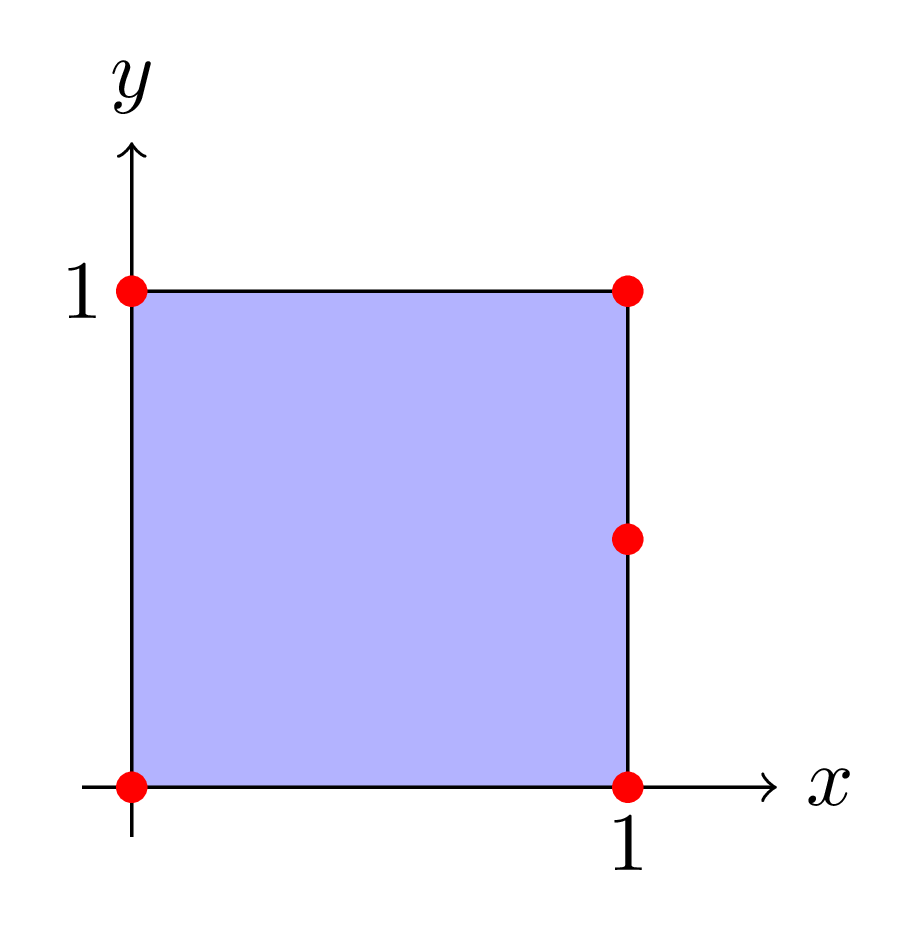
\includegraphics[width=3.9cm]{square-candidates.png}
  %   \end{center}
  % \end{clue}

\end{category}

%======================================================================
\begin{category}{Integrals}

  % Figure from Lab 11 (source in figures/riemann-sum.tex).
  \begin{clue}[say]
    The lines $x=1/2$ and $y=1/2$ split $R = [0,1] \times [0,1]$ into four subrectangles. It is the Riemann sum of $f(x,y) = xy+1$ over $R,$ using the lower left corner of each subrectangle as the sample point.
  \response
    What is $\frac{17}{16}$?
  \solution
    We have $\Delta x=\frac{1}{2}$ and $\Delta y=\frac{1}{2}.$ The lower-left sample points are
    $(0,0),$ $(\frac{1}{2},0),$ $(0,\frac{1}{2}),$ $(\frac{1}{2},\frac{1}{2}).$ So,
    \begin{align*}
    \left(f(0,0)+f\!\left(\tfrac{1}{2},0\right)+f\!\left(0,\tfrac{1}{2}\right)+f\!\left(\tfrac{1}{2},\tfrac{1}{2}\right)\right)\cdot\tfrac{1}{2}\cdot\tfrac{1}{2}
    &=\left(1+1+1+\tfrac{5}{4}\right)\cdot\tfrac{1}{4} \\
    &=\frac{17}{4}\cdot\frac{1}{4}\\
    &=\frac{17}{16}.
    \end{align*}

    \begin{center}
      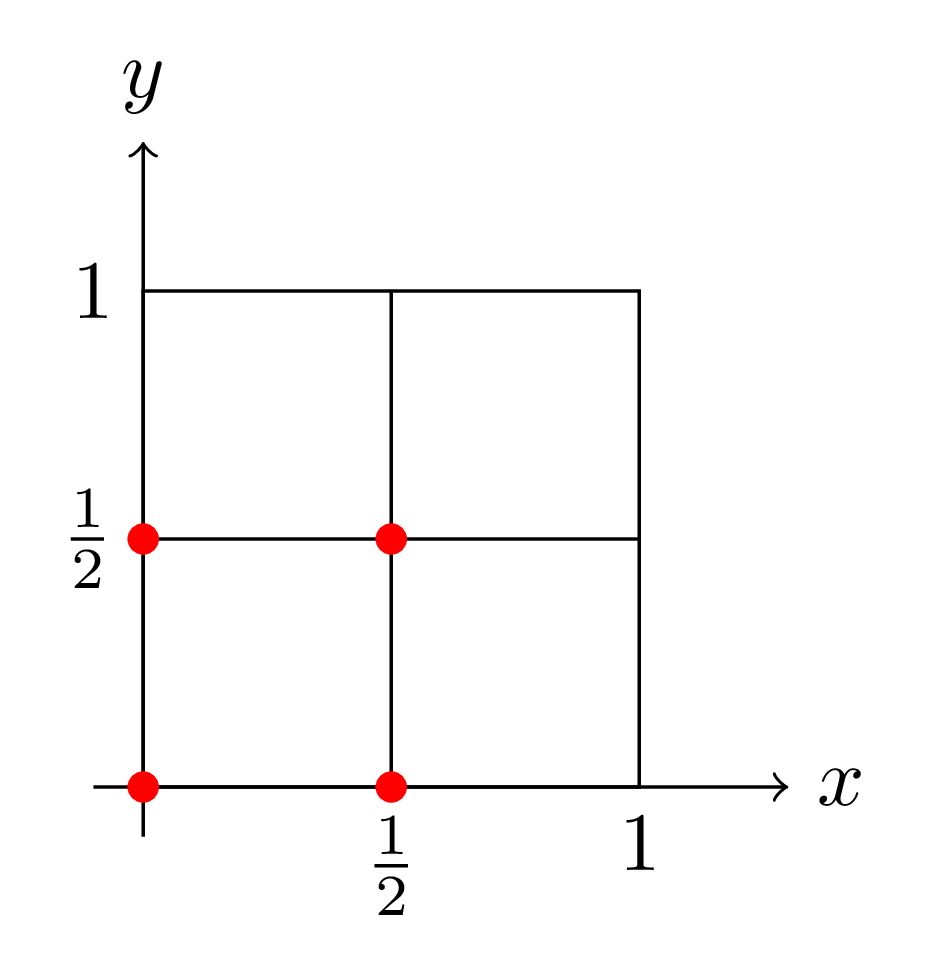
\includegraphics[width=3.9cm]{riemann-sum.png}
    \end{center}
  \end{clue}



  \begin{clue}[write]
    To find $\displaystyle \int x^2\ln x \, dx$ using integration by parts, they are the best choices for $u$ and $dv.$
  \response
    What are $u=\ln x$ and $dv=x^2\,dx$?
  \solution
    Choose $u=\ln x,$ because its derivative is simpler, and $dv=x^2\,dx,$ which is easy to integrate. Then $du=\frac{1}{x}\,dx$ and $v=\frac{x^3}{3},$ so
    \begin{align*}
    \int x^2\ln x\,dx
    &=\frac{x^3}{3}\ln x-\int \frac{x^3}{3}\cdot\frac{1}{x}\,dx \\
    &=\frac{x^3}{3}\ln x-\int \frac{x^2}{3}\,dx \\
    &=\frac{x^3}{3}\ln x-\frac{x^3}{9}+C.
    \end{align*}
    (With $u=x^2$ instead, we would need $v=\int \ln x\,dx,$ which is itself an integration by parts.)
  \end{clue}


  % \begin{clue}[say]
  %   It is the value of $\displaystyle \iint_R (x + \sin y) \; dA,$ where $R = [0,2] \times [0, \pi].$
  % \response
  %   What is $4+2\pi$?
  % \solution
  %   \begin{align*}
  %   \int_0^2\int_0^{\pi}(x+\sin y)\,dy\,dx
  %   &=\int_0^2\left[xy-\cos y\right]_0^{\pi}\,dx \\
  %   &=\int_0^2\bigl((\pi x-\cos\pi)-(0-\cos 0)\bigr)\,dx \\
  %   &=\int_0^2(\pi x+2)\,dx \\
  %   &=\left.\left(\frac{\pi}{2}x^2+2x\right)\right|_0^2 \\
  %   &=2\pi+4.
  %   \end{align*}
  % \end{clue}

  \begin{clue}[say]
    It is the value of $\displaystyle \iiint_E (x^2 + 2y) \; dV,$ where $E = \{(x,y,z) \colon 0 \leq x \leq 1, 0 \leq y \leq 1, 0 \leq z \leq 1\}.$
  \response
    What is $\frac{4}{3}$?
  \solution
    \begin{align*}
    \int_0^1\int_0^1\int_0^1(x^2+2y)\,dx\,dy\,dz
    &=\int_0^1\int_0^1\left[\frac{x^3}{3}+2xy\right]_0^1\,dy\,dz \\
    &=\int_0^1\int_0^1\left(\frac{1}{3}+2y\right)dy\,dz \\
    &=\int_0^1\left[\frac{y}{3}+y^2\right]_0^1\,dz \\
    &=\int_0^1\left(\frac{1}{3}+1\right)dz \\
    &=\left.\frac{4}{3}z\right|_0^1=\frac{4}{3}.
    \end{align*}
  \end{clue}

  % Figure from Lab 11 (source in figures/reverse-order.tex).
  \begin{clue}[write]
    It is $\displaystyle \int_0^1 \int_0^x F(x,y) \; dy\, dx$ with the order of integration reversed.
  \response
    What is $\displaystyle \int_0^1 \int_y^1 F(x,y) \; dx\, dy$?
  \solution
    The region of integration is $\{(x,y)\colon 0\le y\le x\le 1\},$ the triangle below $y=x.$
    Switching the order: $x$ ranges from $y$ to $1,$ and $y$ from $0$ to $1,$ so
    \[
    \int_0^1\int_0^x F(x,y)\,dy\,dx=\int_0^1\int_y^1 F(x,y)\,dx\,dy.
    \]

    \begin{center}
      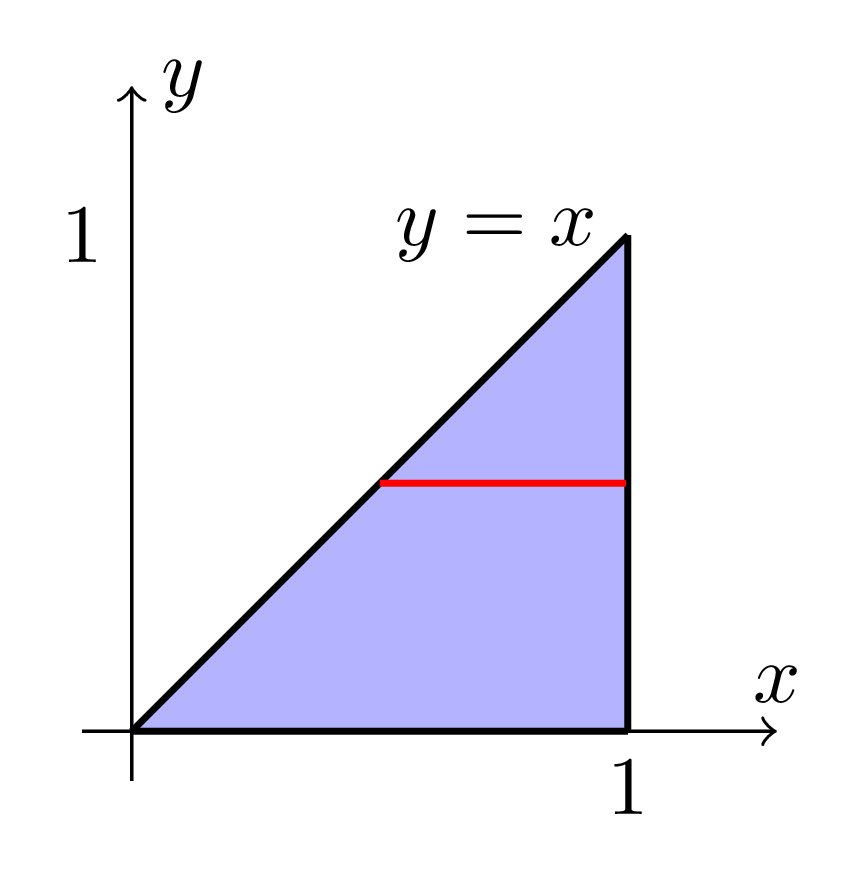
\includegraphics[width=3.6cm]{reverse-order.png}
    \end{center}
  \end{clue}

  % NEW: written by Claude, not from Lab 11.
  % PICTURE: the region between y = x^2 (below) and y = x (above) for 0 <= x <= 1.
  \begin{clue}[say]
    It is the value of $\displaystyle \iint_D x\,dA,$ where $D$ is the region bounded by $y=x$ and $y=x^2.$
  \response
    What is $\frac{1}{12}$?
  \solution
    The curves meet at $x=0$ and $x=1,$ and $x^2\le x$ for $0\le x\le 1.$ So,
    \begin{align*}
    \iint_D x\,dA
    &=\int_0^1\int_{x^2}^{x}x\,dy\,dx \\
    &=\int_0^1 x\left(x-x^2\right)dx \\
    &=\int_0^1\left(x^2-x^3\right)dx \\
    &=\left.\left(\frac{x^3}{3}-\frac{x^4}{4}\right)\right|_0^1 \\
    &=\frac{1}{12}.
    \end{align*}
  \end{clue}

\end{category}

%======================================================================
\begin{category}{Potpourri}

  \begin{clue}[say]
    It is the smallest of the irrational numbers $\pi,$ $e,$ and $\sqrt{2}.$
  \response
    What is $\sqrt{2}$?
  \end{clue}

  \begin{clue}[say]
    It is the second full moon in a single month.
  \response
    What is a blue moon?
  \end{clue}

  % NEW: written by Claude, not from Lab 11.
  \begin{clue}[say]
    It is the volume of a pizza with radius $z$ and thickness $a.$
  \response
    What is $\text{pi}\cdot z\cdot z\cdot a\quad (=\pi z^2 a)$?

  \end{clue}

  % NEW: written by Claude, not from Lab 11.
  \begin{clue}[say]
    This quadric surface, $z=x^2-y^2,$ gives a Pringles chip its shape.
  \response
    What is a hyperbolic paraboloid?

  \end{clue}

  % Retired clue:
  % \begin{clue}[say]
  %   It is a ``mathematical'' car from Acura
  %
  %   (at least the ``LS'' model)
  % \response
  %   What is the ``INTEGRA LS''?
  % \end{clue}

  % Figures from Lab 11 (sources in figures/ant-cube.tex and figures/ant-net.tex).
  \begin{clue}[say]
    An ant sits at one corner of a $1\times 1\times 1$ cube. It is the shortest distance the ant can walk, on the outside of the cube, to reach the opposite corner.
    \begin{center}
      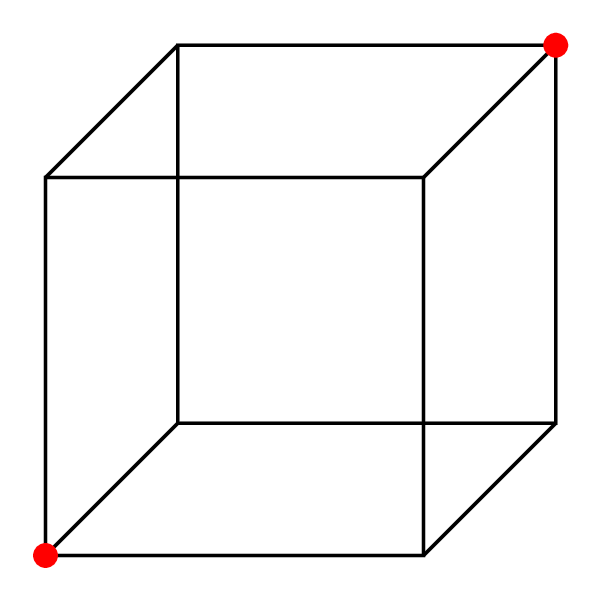
\includegraphics[width=2.5cm]{ant-cube.png}
    \end{center}
  \response
    What is $\sqrt{5}$?
  \solution
    When we unfold the faces of the cube, we see that the ant must walk across a $1\times 2$ rectangle. The ant's shortest path is the straight-line diagonal across this rectangle, which has length $\sqrt{1^2+2^2}=\sqrt{5}.$

    \begin{center}
      \raisebox{-0.5\height}{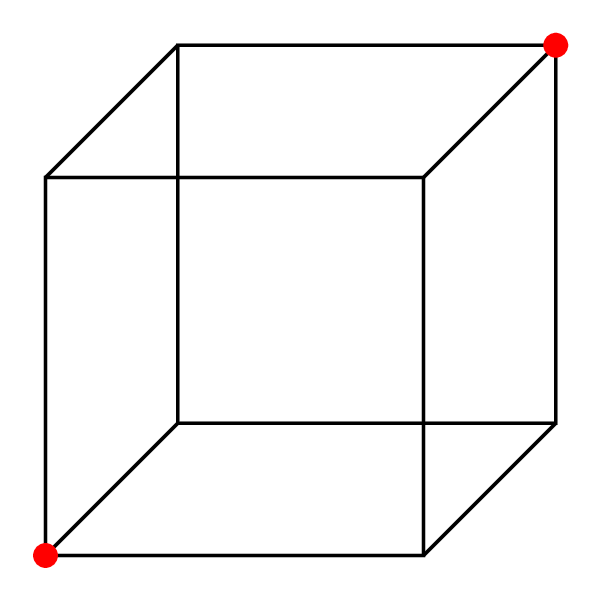
\includegraphics[width=2.5cm]{ant-cube.png}}\hspace{1.5cm}%
      \raisebox{-0.5\height}{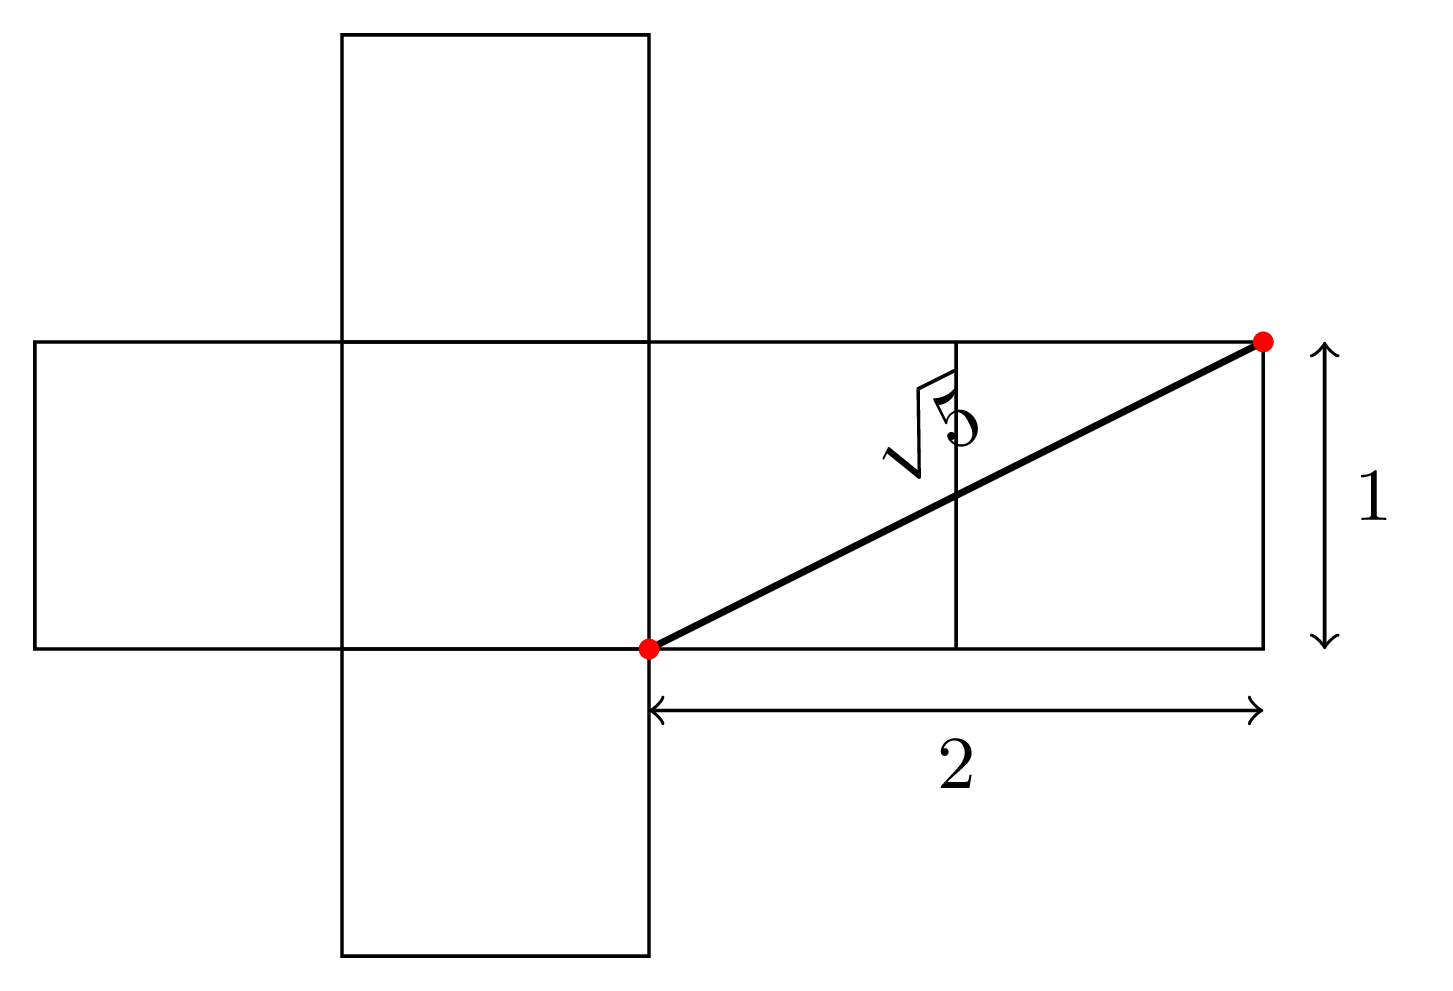
\includegraphics[width=6.2cm]{ant-net.png}}
    \end{center}
  \end{clue}

\end{category}

%======================================================================
% NEW: written by Claude, not from Lab 11.
% PICTURE (optional): the tangent plane above the square R.
\begin{final}{Planes and Volume}
  It is the volume of the solid that lies under the tangent plane to $z=x^2+y^2$ at the point $(1,1,2)$ and above the square $R=[1,2]\times[1,2].$
\response
  What is $4$?
\solution
  We have $f_x(x,y)=2x$ and $f_y(x,y)=2y.$ So, $f_x(1,1)=2$ and $f_y(1,1)=2,$ and the tangent plane is
  \[
  z=2+2(x-1)+2(y-1)=2x+2y-2.
  \]
  This plane is above the $xy$-plane on $R.$ So, the volume is
  \begin{align*}
  \int_1^2\int_1^2(2x+2y-2)\,dy\,dx
  &=\int_1^2\left[2xy+y^2-2y\right]_1^2\,dx \\
  &=\int_1^2(2x+1)\,dx \\
  &=\left.\left(x^2+x\right)\right|_1^2 \\
  &=4.
  \end{align*}
\end{final}

\end{document}
